% =====================================================================
%  Chapitre 0 : Introduction
% =====================================================================
\chapter{Introduction : comprendre le Web et Django}
\label{ch:introduction}

\chapitreresume{Dans ce chapitre, vous découvrez ce qu'est Django, comment une
application web fonctionne et pourquoi le modèle MVT structure tous les projets
Django. Vous préparez aussi votre environnement de travail et vous installez
Django. À la fin, vous êtes prêt à créer le projet \gesibiblio.}

\begin{objectifs}
\begin{itemize}
  \item Expliquer ce qu'est un framework web et ce que Django apporte.
  \item Décrire le trajet d'une requête HTTP, du navigateur à la base de données.
  \item Distinguer le modèle, la vue et le gabarit dans Django.
  \item Présenter les fonctionnalités du projet fil rouge \gesibiblio.
  \item Créer un environnement virtuel et installer Django et Pillow.
  \item Vérifier que l'installation fonctionne.
\end{itemize}
\end{objectifs}

\section{Qu'est-ce que Django ?}

Django est un \textbf{framework web} écrit en Python. Un framework est une boîte à
outils complète : il fournit une structure de projet, un routeur d'URL, un moteur de
gabarits, une couche d'accès à la base de données, une administration automatique,
un système d'authentification et de nombreuses protections contre les failles
courantes.

Sans framework, il faudrait écrire soi-même tout cela : lire les requêtes HTTP,
analyser les formulaires, se connecter à la base, échapper le HTML, gérer les
sessions, hacher les mots de passe, etc. Django s'occupe de ces tâches répétitives
et vous laisse vous concentrer sur ce qui est propre à votre application.

\begin{retenir}
Django suit une philosophie simple : \og ne vous répétez pas \fg{} (DRY, pour
\emph{Don't Repeat Yourself}) et \og tout est inclus \fg{} (batteries included).
Le framework privilégie les conventions claires et la sécurité par défaut.
\end{retenir}

Django est utilisé par des sites de toutes tailles : des journaux en ligne, des
plateformes d'enseignement, des applications de gestion, des API mobiles. Sa
documentation est excellente et sa communauté très active. C'est donc un excellent
premier framework pour apprendre le développement web professionnel.

\section{Comment fonctionne une application web}

Une application web repose sur un dialogue entre un \textbf{client} et un
\textbf{serveur}. Le client est le plus souvent un navigateur : Chrome, Firefox,
Safari ou Edge. Le serveur est un programme qui écoute sur un port et répond aux
demandes.

Le dialogue utilise le protocole HTTP. Une \textbf{requête} contient :
\begin{itemize}
  \item une méthode : \code{GET} pour demander une page, \code{POST} pour envoyer
        des données ;
  \item une URL : par exemple \code{/livres/le-petit-prince/} ;
  \item des en-têtes : le navigateur, la langue, les cookies, etc. ;
  \item parfois un corps : les champs d'un formulaire ou un fichier.
\end{itemize}

Le serveur renvoie une \textbf{réponse} avec un code de statut, des en-têtes et un
corps. Les codes les plus courants sont \code{200} (succès), \code{301} ou
\code{302} (redirection), \code{404} (page introuvable) et \code{500} (erreur du
serveur).

\begin{note}
Quand vous tapez une adresse dans un navigateur, vous envoyez une requête
\code{GET}. Quand vous validez un formulaire de connexion, vous envoyez une requête
\code{POST}. Cette distinction est fondamentale : on ne modifie jamais une donnée
avec une requête \code{GET}.
\end{note}

\section{Le modèle MVT de Django}

Django organise le code selon trois responsabilités : le \textbf{modèle}, la
\textbf{vue} et le \textbf{gabarit}. C'est le modèle MVT, pour
\emph{Model, View, Template}.

\begin{figure}[htbp]
\centering
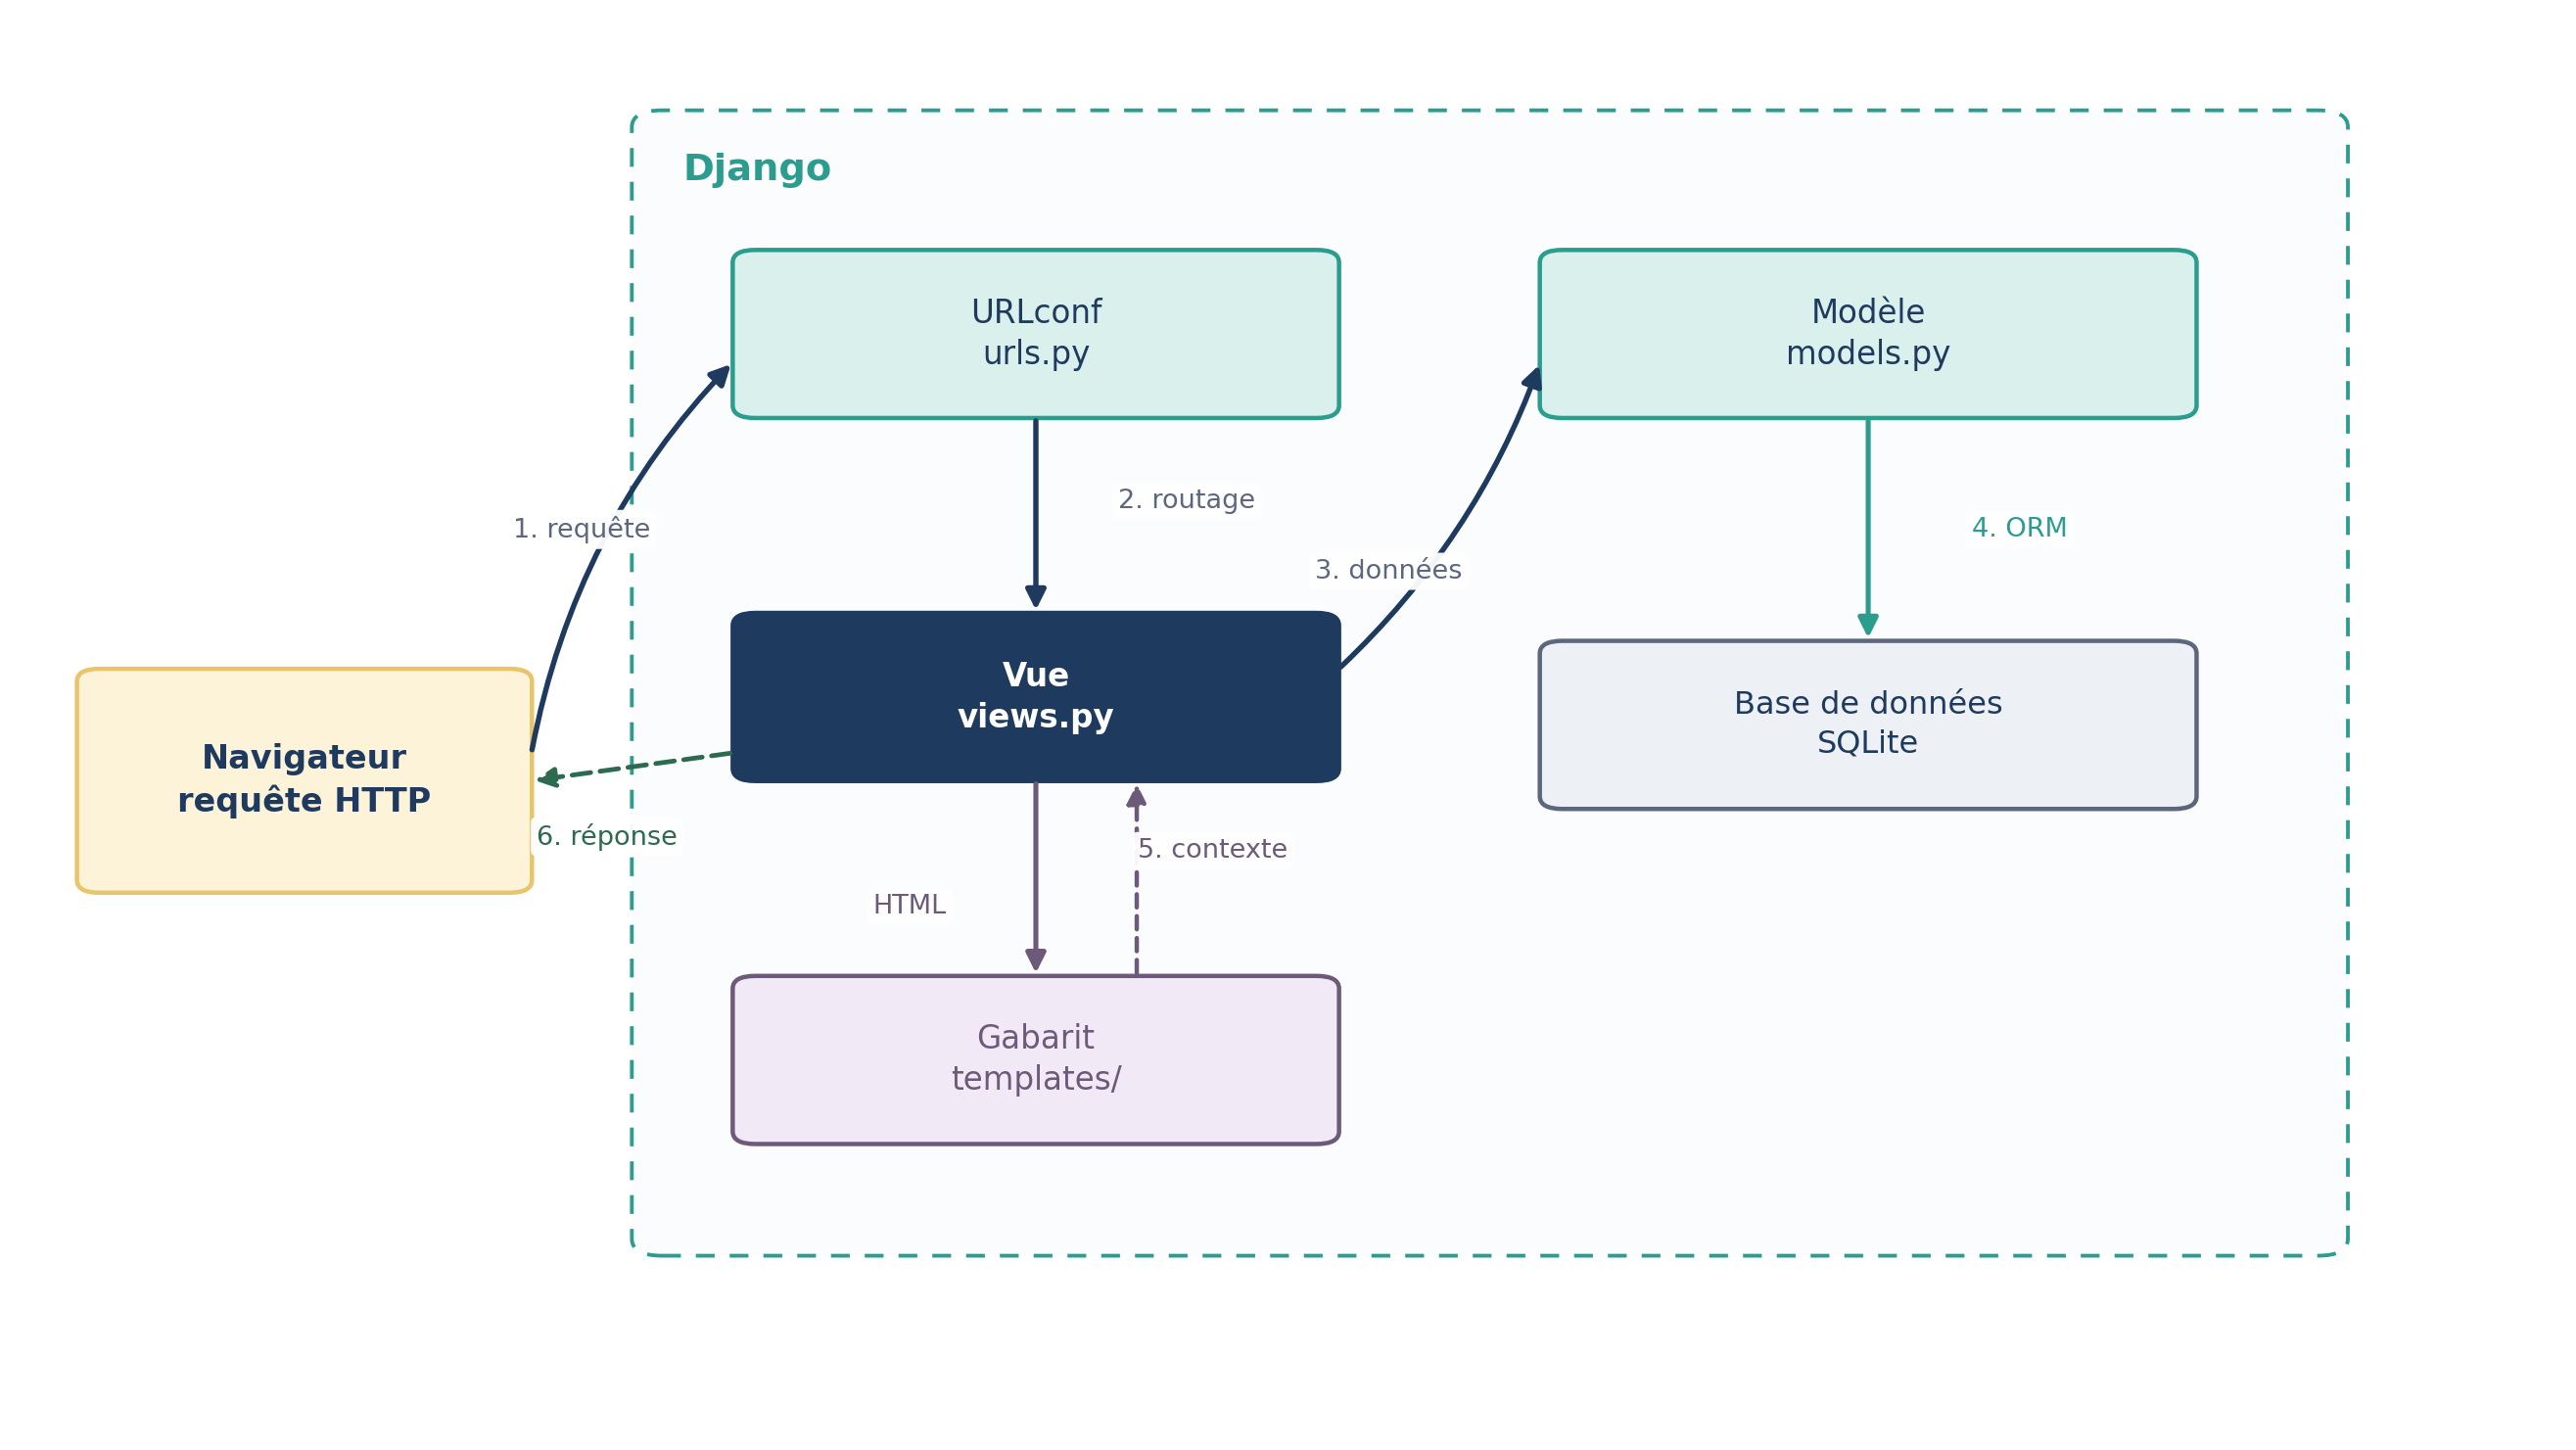
\includegraphics[width=\textwidth]{images/mvt.png}
\caption{Le trajet d'une requête dans Django. La vue orchestre le modèle et le
gabarit, puis renvoie une réponse HTTP.}
\label{fig:mvt}
\end{figure}

\begin{description}[leftmargin=2.6cm,style=nextline]
  \item[Le modèle] Il décrit les données et les règles métier. Un modèle Django est
  une classe Python qui correspond à une table de la base de données. Par exemple,
  \code{Livre} contient un titre, un ISBN, un auteur et un nombre d'exemplaires.
  \item[La vue] C'est une fonction ou une classe Python qui reçoit une requête,
  récupère les données nécessaires, choisit un gabarit et renvoie une réponse. La
  vue contient la logique de la page.
  \item[Le gabarit] C'est un fichier HTML enrichi de balises Django. Il affiche les
  données préparées par la vue. Le gabarit ne doit pas contenir de logique métier.
\end{description}

\begin{attention}
Le vocabulaire de Django peut surprendre si vous venez du modèle MVC classique.
Dans Django, la \og vue \fg{} joue le rôle du contrôleur, et le \og gabarit \fg{}
joue le rôle de la vue. Le tableau suivant clarifie la correspondance.
\end{attention}

\begin{table}[htbp]
\centering
\begin{tabularx}{\textwidth}{L{3.2cm} L{3.2cm} X}
\toprule
\textbf{Django (MVT)} & \textbf{MVC classique} & \textbf{Rôle} \\
\midrule
Modèle & Modèle & Données, relations, règles métier \\
Vue & Contrôleur & Reçoit la requête, prépare les données, choisit la réponse \\
Gabarit & Vue & Présentation HTML, affichage des données \\
\bottomrule
\end{tabularx}
\caption{Correspondance entre MVT et MVC.}
\end{table}

Le trajet complet d'une requête est le suivant :
\begin{enumerate}
  \item le navigateur envoie une requête vers une URL ;
  \item le routeur (\code{urls.py}) associe l'URL à une vue ;
  \item la vue interroge les modèles si nécessaire ;
  \item la vue transmet les données au gabarit ;
  \item le gabarit produit le HTML ;
  \item la vue renvoie une réponse HTTP au navigateur.
\end{enumerate}

\section{Le projet fil rouge : GesiBiblio}

Tout au long du module, vous développez \gesibiblio, une application de gestion de
bibliothèque. Le scénario est simple : une petite bibliothèque veut remplacer son
cahier par un site web. Les lecteurs consultent le catalogue et voient leurs
emprunts. Les bibliothécaires ajoutent des livres, enregistrent les prêts et les
retours.

\begin{table}[htbp]
\centering
\small
\begin{tabularx}{\textwidth}{L{4.2cm} X}
\toprule
\textbf{Fonctionnalité} & \textbf{Description} \\
\midrule
Catalogue & Liste des livres avec recherche par titre, auteur ou ISBN. \\
Fiche livre & Détail d'un livre : auteur, catégories, résumé, couverture. \\
Gestion des livres & Ajout, modification et suppression par les bibliothécaires. \\
Emprunts & Enregistrement d'un prêt, date de retour prévue, retour et retard. \\
Comptes & Inscription, connexion, déconnexion et espace personnel. \\
Permissions & Un lecteur consulte, un bibliothécaire gère le catalogue. \\
Administration & Interface Django pour gérer toutes les données. \\
Design & Interface responsive, lisible sur ordinateur et sur téléphone. \\
\bottomrule
\end{tabularx}
\caption{Fonctionnalités de l'application \gesibiblio.}
\end{table}

Les données principales sont les suivantes :
\begin{itemize}
  \item \textbf{Auteur} : prénom, nom, biographie, date de naissance ;
  \item \textbf{Catégorie} : nom, slug, description ;
  \item \textbf{Livre} : titre, ISBN, auteur, catégories, éditeur, année,
        exemplaires, couverture, statut ;
  \item \textbf{Membre} : utilisateur Django, numéro de carte, téléphone, adresse ;
  \item \textbf{Emprunt} : livre, membre, date d'emprunt, date de retour prévue,
        date de retour effective.
\end{itemize}

\begin{bonne}
Le projet est volontairement petit. Un bon projet de formation n'est pas un projet
gigantesque : c'est un projet que vous comprenez entièrement, que vous pouvez
expliquer et que vous pouvez étendre. \gesibiblio{} couvre l'essentiel de Django
sans vous noyer.
\end{bonne}

\section{Préparer l'environnement de travail}

Avant d'installer Django, vérifiez que Python est disponible. Ouvrez un terminal
(PowerShell sous Windows, Terminal sous macOS ou Linux) et tapez :

\begin{terminal}
python --version
\end{terminal}

Vous devez obtenir une version 3.10 ou supérieure, par exemple :

\begin{terminal}
Python 3.12.7
\end{terminal}

\begin{attention}
Sous Windows, si la commande \code{python} ouvre le Microsoft Store au lieu
d'afficher une version, Python n'est pas installé ou n'est pas dans le
\code{PATH}. Réinstallez Python depuis python.org en cochant \og Add Python to PATH
\fg, puis rouvrez le terminal. Vous pouvez aussi essayer la commande \code{py}.
\end{attention}

\subsection{Créer un dossier de travail}

Créez un dossier pour la formation, puis placez-vous dedans. Par exemple :

\begin{terminal}
mkdir gesibiblio
cd gesibiblio
\end{terminal}

Tout le projet vivra dans ce dossier. Évitez les chemins contenant des caractères
exotiques ou des espaces, surtout sous Windows. Un chemin simple comme
\code{C:\textbackslash{}projets\textbackslash{}gesibiblio} évite bien des surprises.

\subsection{Créer un environnement virtuel}

Un environnement virtuel isole les dépendances du projet. Les paquets installés
pour \gesibiblio{} ne pollueront pas le Python global de votre machine.

\begin{terminal}
python -m venv .venv
\end{terminal}

Activez ensuite l'environnement. Sous Windows :

\begin{terminal}
.venv\Scripts\activate
\end{terminal}

Sous macOS ou Linux :

\begin{terminal}
source .venv/bin/activate
\end{terminal}

Le prompt du terminal commence maintenant par \code{(.venv)}. C'est le signe que
l'environnement est actif.

\begin{attention}
L'activation ne dure que le temps de la session du terminal. Si vous fermez le
terminal, il faut réactiver l'environnement avant de lancer le serveur ou
d'installer un paquet. Si la commande \code{python} ne trouve plus Django, c'est
souvent que l'environnement n'est pas activé.
\end{attention}

\subsection{Installer Django et Pillow}

Mettez pip à jour, puis installez Django et Pillow. Pillow est la bibliothèque
d'images utilisée par Django pour les champs \code{ImageField}.

\begin{terminal}
python -m pip install --upgrade pip
python -m pip install "Django>=5.2,<6.0" Pillow
\end{terminal}

\begin{note}
Les guillemets autour de \code{"Django>=5.2,<6.0"} sont importants dans un
terminal : ils empêchent le shell d'interpréter les caractères \code{>} et
\code{<} comme des redirections. Sous Windows, PowerShell peut aussi avoir besoin
des guillemets.
\end{note}

\subsection{Vérifier l'installation}

\begin{terminal}
python -m django --version
\end{terminal}

La réponse ressemble à \code{5.2.7}. Le numéro exact dépend du moment de votre
installation. L'important est que la commande affiche une version 5.2.x.

Vous pouvez aussi lister les paquets installés :

\begin{terminal}
python -m pip list
\end{terminal}

Vous devez y voir \code{Django} et \code{Pillow}.

\section{Choisir un éditeur de code}

Visual Studio Code est un choix confortable et gratuit. Installez les extensions
suivantes :
\begin{itemize}
  \item \textbf{Python} (Microsoft) : exécution, débogage, complétion ;
  \item \textbf{Django} (Baton) ou \textbf{Django IntelliSense} : aide sur les
        gabarits et les modèles ;
  \item \textbf{GitLens} : historique Git intégré, utile dès que vous versionnez
        votre projet.
\end{itemize}

Ouvrez le dossier \code{gesibiblio} dans VS Code. Le terminal intégré
(\code{Ctrl+ù} ou \code{Ctrl+`}) permet de lancer les commandes sans quitter
l'éditeur.

\begin{bonne}
Prenez l'habitude de travailler avec trois zones : l'arborescence des fichiers à
gauche, le code au centre et le terminal en bas. Cette organisation réduit les
allers-retours et rend les erreurs plus faciles à repérer.
\end{bonne}

\section{Comment utiliser ce module}

Chaque chapitre contient trois types de blocs :
\begin{itemize}
  \item les blocs \textbf{Terminal}, pour les commandes ;
  \item les blocs \textbf{Code}, avec le chemin du fichier et des numéros de ligne ;
  \item les encadrés de méthode, d'attention et d'exercice.
\end{itemize}

Le code est cumulatif. Le fichier \code{catalogue/views.py} du chapitre 7 contient
les fonctions écrites aux chapitres précédents, parfois complétées. Si vous sautez
un chapitre, revenez au fichier complet fourni dans la correction ou dans le bilan
final.

\begin{retenir}
Django n'est pas une suite de recettes magiques. C'est un framework cohérent :
une URL appelle une vue, la vue utilise des modèles, le modèle parle à la base, et
le gabarit affiche le résultat. Si vous gardez ce trajet en tête, vous saurez
toujours où chercher quand quelque chose ne fonctionne pas.
\end{retenir}

\section{Exercices}

\begin{exercice}[ : vérifier son environnement]
Réalisez les opérations suivantes et notez les résultats :
\begin{enumerate}
  \item afficher la version de Python ;
  \item créer un environnement virtuel nommé \code{.venv} ;
  \item activer cet environnement ;
  \item installer Django et Pillow ;
  \item afficher la version de Django ;
  \item désactiver l'environnement avec la commande \code{deactivate}.
\end{enumerate}
\end{exercice}

\begin{correction}
\begin{terminal}
python --version
python -m venv .venv
.venv\Scripts\activate
python -m pip install "Django>=5.2,<6.0" Pillow
python -m django --version
deactivate
\end{terminal}

Sous macOS ou Linux, remplacez la troisième ligne par
\code{source .venv/bin/activate}. La commande \code{deactivate} fonctionne sur
tous les systèmes.
\end{correction}

\begin{exercice}[ : expliquer le MVT]
Sans regarder le cours, expliquez en trois phrases le rôle du modèle, de la vue et
du gabarit. Puis décrivez ce qui se passe quand un visiteur demande la fiche du
livre \og Le Petit Prince \fg.
\end{exercice}

\begin{correction}
Le modèle décrit les données et les règles métier. La vue reçoit la requête,
interroge le modèle et choisit un gabarit. Le gabarit produit le HTML affiché.

Pour la fiche du livre, le navigateur appelle une URL du type
\code{/livres/le-petit-prince/}. Le routeur associe cette URL à la vue
\code{livre\_detail}. La vue cherche le livre dans la base avec son slug, puis
transmet l'objet \code{livre} au gabarit \code{detail.html}. Le gabarit affiche le
titre, l'auteur et le résumé, et la vue renvoie la page HTML au navigateur.
\end{correction}

\begin{retenir}
\begin{itemize}
  \item Django est un framework Python complet, sécurisé et structuré.
  \item Une application web échange des requêtes et des réponses HTTP.
  \item Le modèle MVT sépare les données, la logique et la présentation.
  \item Le projet fil rouge \gesibiblio{} sera construit brique par brique.
  \item Un environnement virtuel isole les dépendances du projet.
\end{itemize}
\end{retenir}
